% Created 2023-12-03 So 16:34
% Intended LaTeX compiler: pdflatex
\documentclass[11pt]{article}
\usepackage[utf8]{inputenc}
\usepackage{lmodern}
\usepackage[T1]{fontenc}
\usepackage{textcomp}
\usepackage{graphicx}
\usepackage{longtable}
\usepackage{wrapfig}
\usepackage{rotating}
\usepackage[normalem]{ulem}
\usepackage{amsmath}
\usepackage{amssymb}
\usepackage{capt-of}
\usepackage{hyperref}
\usepackage{verbatim}
\usepackage{listings}
\usepackage{underscore}
\author{Leon Schwarzäugl}
\date{\today}
\title{Computational Science on Many-Core Architectures \\Exercise 6}
\hypersetup{
 pdfauthor={Leon Schwarzäugl},
 pdftitle={Computational Science on Many-Core Architectures, Exercise 7},
 pdfkeywords={},
 pdfsubject={},
 pdfcreator={Emacs 30.0.50 (Org mode 9.6.12)},
 pdflang={English}}
\begin{document}
\maketitle
The code for all tasks can be found at: \url{https://github.com/Swarsel/CSE_TUWIEN/tree/main/WS2023/Many-Core%20Architectures/e6}
\newpage
\section{Inclusive and Exclusive Scan}

\subsection{(1)}


\subsubsection{scan_kernel_1}
This kernel starts by (after loading variables that are useful to be declared as well as initializing shared memory) for each section, loading data from a const vector X into the (private) local variable my_value. \\
Afterwards an inclusive scan is performed by storing the value of my_buffer in the respective shared_buffer entry for each thread, and afterwards adding to my_value the value of a thread previous to it, depending on the current stride; after concluding the strides, all threads write the updated my_value into the respective shared_buffer entry. \\
In the end, the last thread of each block now holds the sum of the elements belonging to the block.
\\
Now, the beginning of each block is set to \(0\) for the first thread and the other threads take the value of the thread with index \(i - 1\) ('one to the left'). Then my_value is written to Y. Finally, we compute the block_offset - this is the sum of each thread in a block - we write it to the carries in the entry respective to the block.

\subsubsection{scan_kernel_2}

We now use these carries to perform the exclusive scan on the carries.
Notably only one block is launched for this kernel.
After that we again add the elements towards the last element using a shared_buffer and then  right-shift with a \(0\) in the first position.

This result is written to the carry array, which now holds the offsets in a summed manner (ascending 'from left to right').

\subsubsection{scan_kernel_3}

This kernel simply adds the applying offsets. The exclusive scan is finished and the result is stored in Y.

\subsection{(2)}

This task was achieved by letting the same kernels run as before, but then copying back the values with the shift 'remedied' and the last value computed by hand on the CPU.

\subsection{(3)}

This was accomplished by commenting out line 43 of the original code (where the shift happens).

\subsection{(4)}

\textit{Note:} Benchmarked for each version was the time until the result is available on the host. The result would have been skewed if I would have just taken the time until the result is available \textit{somewhere}, since one of the versions has a computation on the CPU and would hence need an extra cudaMemcpy.

We can see that the execution times are very similar; for low N it seems that the problem size has no considerable bearing on the run length and we are mostly measuring overhead. Even for bigger N there is no real difference in run time.

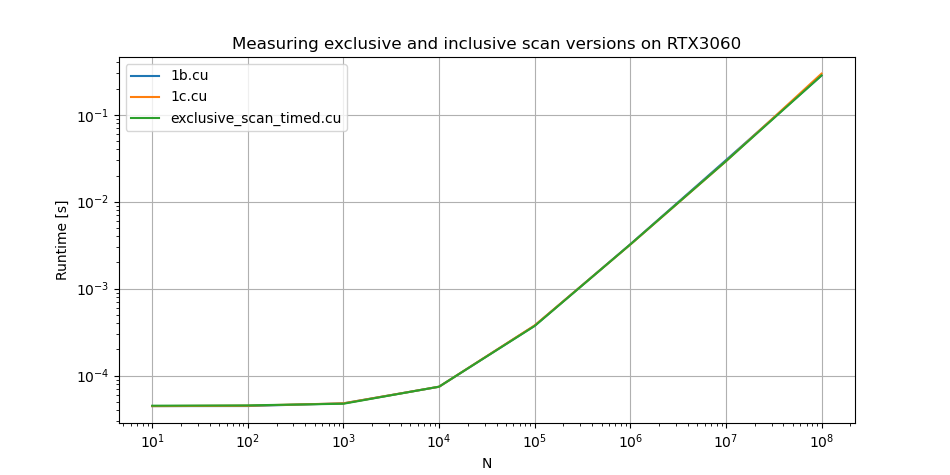
\includegraphics[scale=0.5]{plots/1global.png}

When zooming very far in, we get a more detailed picture (the measurements were, as always, performed 14 times, with the lowest and highest two times omitted and over the rest averaged):

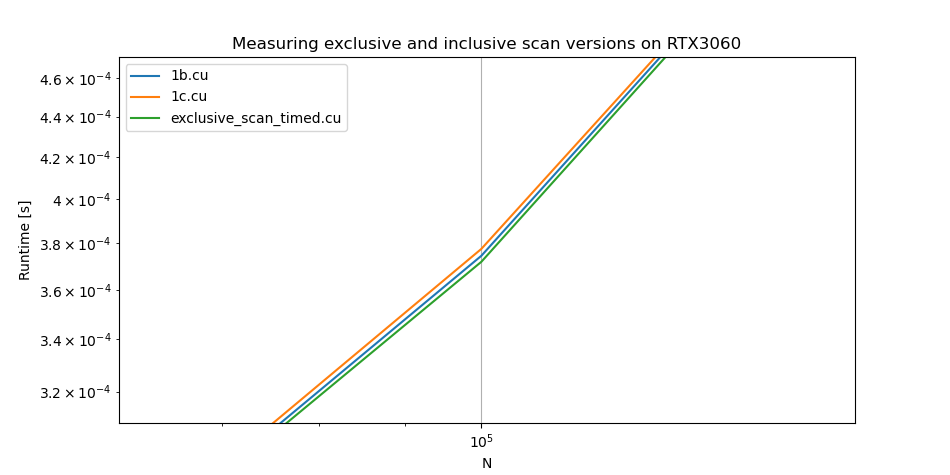
\includegraphics[scale=0.5]{plots/1zoom.png}

This would suggest that the 'reusing-exclusive-scan' and exclusive-scan versions perform faster than the 'exclusive-scan-changed' vesion. I find this very surprising, considering that the '[...]-changed' version has strictly less operations to persorm than the rest. Maybe I made an error here somewhere, but I cannot seem to find one.
\pagebreak
\section{Finite Differences on the GPU}

\subsection{(1)}

The following kernel was implemented, nearly verbatim to the slides :)

\begin{verbatim}

__global__ void count_nnz(int *row_offsets, int N, int M) {
  for (int row = blockDim.x * blockIdx.x + threadIdx.x;
       row < N*M;
       row += gridDim.x * blockDim.x)
    {
      int nnz_for_this_node = 1;
      int i = row / N;
      int j = row % N;
      if (i > 0) nnz_for_this_node += 1;
      if (j > 0) nnz_for_this_node += 1;
      if (i < N-1) nnz_for_this_node += 1;
      if (j < M-1) nnz_for_this_node += 1;
      row_offsets[row] = nnz_for_this_node;
    }
}

\end{verbatim}

\subsection{(2)}

This was achieved by first calling the aforementioned kernel and then passing it as an input to the exclusive scan:

\begin{verbatim}

  count_nnz<<<256, 256>>>(cuda_nnz, N, M);
  exclusive_scan(cuda_nnz, cuda_csr_rowoffsets, (N * M + 1));

\end{verbatim}
\pagebreak
\subsection{(3)}

This kernel was only slightly adjusted for the other directions compared to the slides:
\begin{verbatim}
__global__ void assembleA(int *row_offsets, int *col_indices, double *values, int N, int M) {
  for (int row = blockDim.x * blockIdx.x + threadIdx.x;
       row < N*M;
       row += gridDim.x * blockDim.x) {
    int i = row / N;
    int j = row % N;
    int this_row_offset = row_offsets[row];
    // diagonal entry
    col_indices[this_row_offset] = i * N + j;
    values[this_row_offset] = 4;
    this_row_offset += 1;
    if (i > 0) { // bottom neighbor
      col_indices[this_row_offset] = (i-1) * N + j;
      values[this_row_offset] = -1;
      this_row_offset += 1;
    }
    if (j > 0) { /* similarly */
      col_indices[this_row_offset] = i + N * (j-1);
      values[this_row_offset] = -1;
      this_row_offset += 1;
    }
    if (i < N-1) { /* similarly */
      col_indices[this_row_offset] = (i+1) * N + j;
      values[this_row_offset] = -1;
      this_row_offset += 1;
    }
    if (j < M-1) { /* similarly */
      col_indices[this_row_offset] = i + N * (j+1);
      values[this_row_offset] = -1;
      this_row_offset += 1;
    }
  }
}

\end{verbatim}

\subsection{(4)}

This was implemented an can be found in the respective 2_*.cu files. There are several versions for timing the different parameters. For timing the assemblies, the following CG code was commented out to save useless computation - I checked correctness however.

\subsection{(5)}

We can see that the GPU version is clearly a lot faster in setting up the matrix, while the CPU assembly is still the main culprit for pushing that version towards the \(30\mathrm{s}\) limit. I only measured the CG runtime on one of the versions to save on execution time on the remote host, since (like last exercise) I was often times getting the '[errno:16] device busy' error. Also that code is the exact same for both versions (at least if I understood the assignment correctly) since they both just run the GPU code that we tried to implement last week.

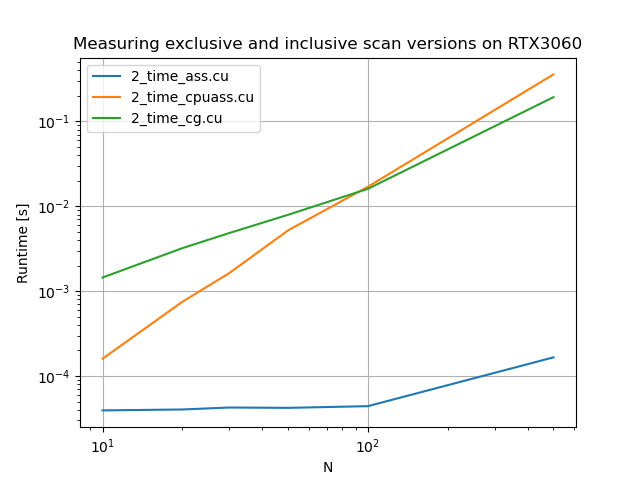
\includegraphics[scale=0.8]{plots/2comp.png}
\pagebreak
\section{Bonus Point: Visualize Result}

The poisson problem was solved for a \( 100 \times 100\) system using the code from above and is visualized below!

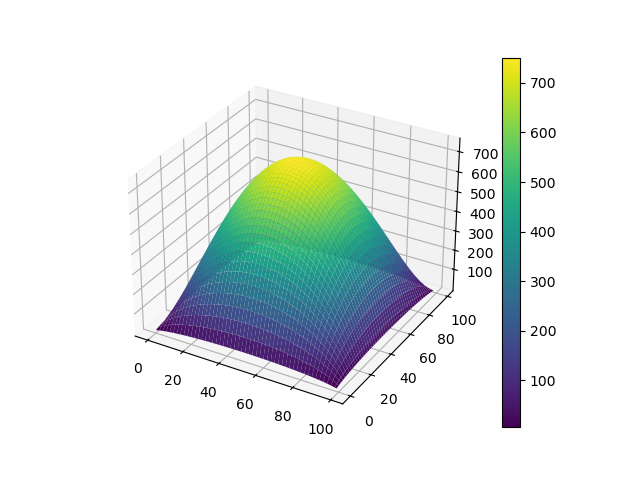
\includegraphics{plots/surf.png}

\end{document}
